\documentclass[11pt,letterpaper]{article}

\usepackage[spanish,es-noshorthands]{babel}
\usepackage{fontspec}
\setmainfont{Source Serif Pro}
\usepackage{microtype}
\usepackage{geometry}
\usepackage{booktabs}
\usepackage{tabularx}
\usepackage{enumitem}
\usepackage{xcolor}
\usepackage{graphicx}
\usepackage{csquotes}
\usepackage{amsmath}
\usepackage{siunitx}
\usepackage{tikz}
\usetikzlibrary{arrows.meta,positioning,shapes.geometric}
\usepackage{xurl}
\usepackage[hidelinks]{hyperref}
\usepackage[backend=biber,style=apa,sorting=nyt]{biblatex}
\DeclareLanguageMapping{spanish}{spanish-apa}

\geometry{margin=2.5cm}
\setlength{\emergencystretch}{1em}
\setlength{\parindent}{0pt}
\setlength{\parskip}{0.65em}
\setlist{nosep}
\addbibresource{referencias.bib}
\AtBeginBibliography{\sloppy}

\sisetup{
  output-decimal-marker = {,},
  group-separator = {.},
  group-minimum-digits = 4,
  per-mode = symbol,
  detect-all
}
\DeclareSIUnit{\ton}{ton}
\DeclareSIUnit{\lb}{lb}
\DeclareSIUnit{\kWh}{kWh}

\title{\textbf{Fundición del acero en un horno de arco eléctrico}\\
\large Límite termodinámico del consumo eléctrico y desempeño alcanzado en el
año 2000}
\author{Carlos Luis Rojas Aragonés\\
Gestión del Desarrollo Tecnológico}
\date{29 de julio de 2026}

\begin{document}

\maketitle

\section{Planteamiento}

El objetivo de este trabajo es doble. Primero, estimar el \textbf{límite teórico
más bajo} de consumo de electricidad necesario para fundir una tonelada de acero,
expresado en \si{\kWh\per\ton}. Segundo, comparar ese límite con el desempeño
real del horno de arco eléctrico (\emph{Electric Arc Furnace}, EAF) en el año
2000, para determinar qué parte del recorrido posible había completado la
tecnología después de tres décadas de mejora continua.

El límite se calcula a partir de la termodinámica del cambio de estado: la
energía mínima para fundir un sólido no depende del diseño del horno, sino de
las propiedades del material. Ese valor funciona como una \emph{frontera física}
—el techo de la curva en S de la tecnología \parencite{foster1986}— y por lo
tanto es una referencia legítima para juzgar cuánta mejora quedaba disponible.

\begin{table}[ht]
  \centering
  \small
  \caption{Datos de partida proporcionados para el cálculo.}
  \label{tab:datos}
  \begin{tabularx}{\textwidth}{@{}>{\raggedright\arraybackslash}X l l@{}}
    \toprule
    \textbf{Parámetro} & \textbf{Símbolo} & \textbf{Valor} \\
    \midrule
    Temperatura de fusión del acero & $T_{final}$ & \SI{1500}{\celsius} \\
    Temperatura inicial de la carga (supuesto) & $T_{inicial}$ & \SI{25}{\celsius} \\
    Calor específico del acero & $c$ & \SI{0.466}{\joule\per\gram\per\celsius} \\
    Calor latente de fusión del acero & $L$ & \SI{276}{\joule\per\gram} \\
    Masa de referencia (una tonelada) & $m$ & \SI{1e6}{\gram} \\
    Equivalencia energética & --- & \SI{3600}{\kilo\joule} $=$ \SI{1}{\kWh} \\
    \bottomrule
  \end{tabularx}
\end{table}

Una precisión sobre el enunciado: los datos entregados (calor específico y calor
latente) corresponden al \textbf{acero}, no a la escoria. El cálculo que sigue
estima, por tanto, la energía mínima para llevar una tonelada de carga metálica
sólida —chatarra de acero— hasta su punto de fusión y cambiarla de fase, que es
justamente la magnitud comparable con la figura de mérito
\si{\kWh\per\ton} del horno de arco eléctrico.

\section{Modelo de cálculo}

La energía total necesaria para fundir un material sólido es la suma de dos
términos: la energía que eleva su temperatura hasta el punto de fusión (calor
sensible) y la energía que produce el cambio de fase a esa misma temperatura
(calor latente):

\begin{equation}
  Q_{total} = Q_{calor} + Q_{calor\ latente}
  \label{eq:total}
\end{equation}

\begin{equation}
  Q_{calor} = m \cdot c \cdot (T_{final} - T_{inicial})
  \label{eq:sensible}
\end{equation}

\begin{equation}
  Q_{calor\ latente} = m \cdot L
  \label{eq:latente}
\end{equation}

donde $m$ es la masa en gramos, $c$ el calor específico en
\si{\joule\per\gram\per\celsius}, $T$ la temperatura en \si{\celsius} y $L$ el
calor latente en \si{\joule\per\gram}. La conversión a unidades comerciales de
energía eléctrica utiliza la equivalencia \SI{3600}{\kilo\joule} $=$
\SI{1}{\kWh}.

El modelo supone un proceso ideal: toda la energía entregada se transfiere al
metal, sin pérdidas por radiación, gases de escape, refrigeración de paneles,
escoria ni sobrecalentamiento. Es precisamente esa idealidad la que convierte al
resultado en un \emph{límite inferior}: ningún horno real puede consumir menos.

\section{Cálculo del límite teórico}

\subsection*{01. Calor sensible}

Aplicando la ecuación~\eqref{eq:sensible} con $\Delta T = 1500 - 25 =
\SI{1475}{\celsius}$:

\begin{align}
  Q_{calor} &= \SI{1e6}{\gram} \times \SI{0.466}{\joule\per\gram\per\celsius}
    \times \SI{1475}{\celsius} \nonumber \\
  &= \SI{687350000}{\joule} = \SI{687350}{\kilo\joule}
\end{align}

\subsection*{02. Calor latente}

Aplicando la ecuación~\eqref{eq:latente}:

\begin{align}
  Q_{calor\ latente} &= \SI{1e6}{\gram} \times \SI{276}{\joule\per\gram}
    \nonumber \\
  &= \SI{276000000}{\joule} = \SI{276000}{\kilo\joule}
\end{align}

\subsection*{03. Energía total y conversión a kWh}

\begin{equation}
  Q_{total} = \SI{687350}{\kilo\joule} + \SI{276000}{\kilo\joule}
  = \SI{963350}{\kilo\joule}
\end{equation}

\begin{equation}
  E = \frac{\SI{963350}{\kilo\joule}}{\SI{3600}{\kilo\joule\per\kWh}}
  = \SI{267.6}{\kWh\per\ton}
  \label{eq:limite}
\end{equation}

\begin{quote}
\textbf{Resultado.} El límite teórico más bajo de consumo de electricidad para
fundir una tonelada de acero es de aproximadamente
\textbf{\SI{268}{\kWh\per\ton}}.
\end{quote}

De ese total, el calor sensible representa el \SI{71.4}{\percent}
(\SI{191.0}{\kWh\per\ton}) y el calor latente el \SI{28.6}{\percent}
(\SI{76.7}{\kWh\per\ton}). El resultado es poco sensible a la temperatura
inicial supuesta: partir de \SI{0}{\celsius} eleva el límite a
\SI{270.8}{\kWh\per\ton} y partir de \SI{20}{\celsius} lo sitúa en
\SI{268.2}{\kWh\per\ton}, una variación inferior al \SI{1.2}{\percent}.

\section{Desempeño del horno de arco eléctrico en 2000}

La Figura~\ref{fig:merito} presenta la evolución de tres figuras de mérito de la
fundición de acero entre 1970 y 2000: el tiempo \emph{tap-to-tap}, el consumo
eléctrico y el consumo de electrodos. El Cuadro~\ref{tab:serie} recoge los
mismos valores en forma numérica.\footnote{En el eje horizontal de la figura
original el sexto punto aparece rotulado como 1990 por segunda vez; por la
progresión quinquenal de la serie corresponde a 1995, y así se registra en el
Cuadro~\ref{tab:serie}.}

\begin{figure}[ht]
  \centering
  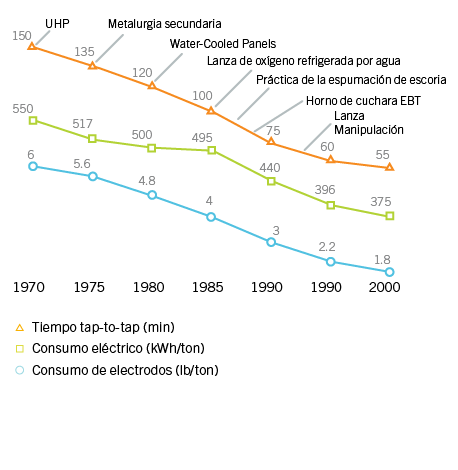
\includegraphics[width=0.86\textwidth]{images/figuras-merito-eaf.png}
  \caption{Tres figuras de mérito en la fundición de acero (1970--2000) y las
  innovaciones asociadas a cada tramo de mejora. Figura proporcionada en el
  material del curso.}
  \label{fig:merito}
\end{figure}

\begin{table}[ht]
  \centering
  \small
  \caption{Serie de las tres figuras de mérito y comparación con el límite
  teórico calculado.}
  \label{tab:serie}
  \begin{tabularx}{\textwidth}{@{}l *{7}{>{\centering\arraybackslash}X}@{}}
    \toprule
    & \textbf{1970} & \textbf{1975} & \textbf{1980} & \textbf{1985}
    & \textbf{1990} & \textbf{1995} & \textbf{2000} \\
    \midrule
    Tiempo \emph{tap-to-tap} (min) & 150 & 135 & 120 & 100 & 75 & 60 & 55 \\
    Consumo eléctrico (kWh/ton) & 550 & 517 & 500 & 495 & 440 & 396 & 375 \\
    Consumo de electrodos (lb/ton) & 6,0 & 5,6 & 4,8 & 4,0 & 3,0 & 2,2 & 1,8 \\
    \midrule
    Eficiencia frente al límite (\si{\percent}) & 48,7 & 51,8 & 53,5 & 54,1 & 60,8 & 67,6
      & 71,4 \\
    Exceso sobre el límite (kWh/ton) & 282 & 249 & 232 & 227 & 172 & 128
      & 107 \\
    \bottomrule
  \end{tabularx}
\end{table}

En el año 2000 el horno de arco eléctrico consumía \SI{375}{\kWh\per\ton}. La
comparación con el límite de la ecuación~\eqref{eq:limite} arroja:

\begin{itemize}
  \item \textbf{Exceso absoluto:} $375 - 267{,}6 = \SI{107.4}{\kWh\per\ton}$ por
    encima del mínimo termodinámico.
  \item \textbf{Exceso relativo:} el consumo real era un \SI{40.1}{\percent}
    superior al límite teórico ($375 / 267{,}6 = 1{,}40$).
  \item \textbf{Eficiencia termodinámica:} $267{,}6 / 375 =
    \SI{71.4}{\percent}$ de la energía consumida correspondía al mínimo
    inevitable.
  \item \textbf{Recorrido restante:} solo quedaba un \SI{28.6}{\percent} de
    reducción posible sobre el valor del año 2000, frente al
    \SI{51.3}{\percent} que quedaba disponible en 1970.
\end{itemize}

Dicho de otro modo: en 1970 el horno consumía \num{2.06} veces el mínimo
teórico; en 2000 consumía \num{1.40} veces ese mínimo. La tecnología recorrió
aproximadamente el \SI{62}{\percent} de la distancia que la separaba de su
frontera física.

\section{Interpretación desde la gestión tecnológica}

\subsection*{01. Las tres figuras de mérito no mejoran al mismo ritmo}

Entre 1970 y 2000, el tiempo \emph{tap-to-tap} cayó un \SI{63.3}{\percent} (de
150 a 55 minutos) y el consumo de electrodos un \SI{70}{\percent} (de 6,0 a 1,8
lb/ton), mientras el consumo eléctrico se redujo solo un \SI{31.8}{\percent} (de
550 a 375 kWh/ton). Esta asimetría no es casual: el consumo eléctrico es la
única de las tres métricas que tropieza con una barrera termodinámica dura y
cercana. Las otras dos dependen de la logística del proceso, de la calidad de los
materiales y del control, donde el margen de mejora era mucho mayor en términos
relativos.

Para la gestión tecnológica, la lección es que \textbf{no todas las figuras de
mérito de una misma tecnología están igual de cerca de su límite}. Evaluar el
potencial restante exige calcular la frontera de cada una por separado
\parencite{foster1986}.

\subsection*{02. La mejora fue acumulativa e incremental}

Las innovaciones señaladas en la Figura~\ref{fig:merito} —transformadores de
ultra alta potencia (UHP), metalurgia secundaria, paneles refrigerados por agua,
lanza de oxígeno refrigerada por agua, práctica de espumación de escoria, horno
de cuchara y colada excéntrica por el fondo (EBT), y manipuladores de lanza— no
constituyen una discontinuidad tecnológica. Ninguna sustituyó al horno de arco
eléctrico: todas lo refinaron. Es el patrón clásico de una tecnología que ya
alcanzó su diseño dominante y entra en una fase de innovación incremental de
proceso \parencite{utterback1994,madias2014}.

El resultado agregado es una reducción del \SI{1.27}{\percent} anual compuesto
en el consumo eléctrico. Si esa tasa se hubiera mantenido indefinidamente, el
consumo alcanzaría el límite teórico hacia 2026. En la práctica no puede
ocurrir: la curva se aplana asintóticamente y el costo marginal de cada
kWh adicional ahorrado crece de forma acelerada conforme se aproxima a la
frontera.

\subsection*{03. Implicación estratégica}

Con un \SI{71.4}{\percent} de eficiencia termodinámica en el año 2000, seguir
invirtiendo en optimizar el consumo eléctrico del EAF ofrecía retornos
decrecientes. Las oportunidades de creación de valor se desplazaban hacia otros
frentes: reducir el tiempo de ciclo, disminuir el costo de los insumos, mejorar
la calidad del producto, aprovechar el calor residual, o cambiar el vector
energético (por ejemplo, hacia electricidad de bajo carbono o hacia rutas de
reducción directa con hidrógeno). La proximidad al límite físico es, en sí
misma, una señal de que la próxima mejora significativa no vendrá de la misma
curva.

\begin{figure}[ht]
  \centering
  \begin{tikzpicture}[
    node distance=5mm,
    bloque/.style={draw, rounded corners, align=center, minimum height=11mm,
      text width=0.20\textwidth},
    flecha/.style={-{Stealth[length=2.2mm]}, thick}
  ]
    \node[bloque, fill=blue!6] (limite) {Límite teórico\\
      \SI{268}{\kWh\per\ton}};
    \node[bloque, right=of limite, fill=orange!10] (y1970) {EAF 1970\\
      \SI{550}{\kWh\per\ton}\\(\SI{48.7}{\percent})};
    \node[bloque, right=of y1970, fill=orange!14] (y2000) {EAF 2000\\
      \SI{375}{\kWh\per\ton}\\(\SI{71.4}{\percent})};
    \node[bloque, right=of y2000, fill=green!9] (brecha) {Brecha restante\\
      \SI{107}{\kWh\per\ton}};
    \draw[flecha] (limite) -- (y1970);
    \draw[flecha] (y1970) -- (y2000);
    \draw[flecha] (y2000) -- (brecha);
  \end{tikzpicture}
  \caption{Posición del horno de arco eléctrico respecto de su frontera
  termodinámica. Elaboración propia.}
  \label{fig:brecha}
\end{figure}

\section{Precisiones y limitaciones del cálculo}

El valor de \SI{268}{\kWh\per\ton} responde exactamente a los datos del
enunciado, pero conviene explicitar cuatro supuestos que afectan su
interpretación.

\begin{enumerate}
  \item \textbf{Calor específico constante.} El valor
    \SI{0.466}{\joule\per\gram\per\celsius} corresponde al acero a temperatura
    ambiente. El calor específico del hierro aumenta con la temperatura y
    presenta discontinuidades asociadas a sus transformaciones alotrópicas y
    magnéticas. Un cálculo entálpico riguroso sitúa la energía mínima para
    llevar chatarra a acero líquido en un orden de magnitud superior, cercano a
    \SI{1.3}{\giga\joule\per\ton} (unos \SI{360}{\kWh\per\ton})
    \parencite{fruehan2000}. El presente cálculo, por tanto, es un límite
    inferior conservador.
  \item \textbf{Sin sobrecalentamiento.} Un horno real no cuela el acero a su
    punto de fusión, sino entre \SI{1600}{\celsius} y \SI{1650}{\celsius} para
    permitir el transporte y la colada. Incorporando ese sobrecalentamiento con
    los mismos datos, el mínimo sube a \SI{280.5}{\kWh\per\ton} y
    \SI{287.0}{\kWh\per\ton} respectivamente.
  \item \textbf{Sin escoria ni pérdidas.} El cálculo ignora la energía para
    fundir la escoria y los fundentes, las pérdidas por gases de escape,
    radiación y refrigeración, y el consumo de los sistemas auxiliares, que en
    conjunto explican la mayor parte de la brecha observada
    \parencite{worrell2010}.
  \item \textbf{La electricidad no es la única fuente de energía.} El EAF
    moderno aporta una fracción sustancial de su energía por vía química
    —quemadores oxicombustible, inyección de oxígeno y carbón, espumación de
    escoria—, precisamente algunas de las innovaciones señaladas en la
    Figura~\ref{fig:merito}. Por esa razón, la figura de mérito
    \si{\kWh\per\ton} \emph{eléctricos} puede en principio descender por debajo
    del mínimo termodinámico total sin violar la termodinámica: parte del
    aporte simplemente deja de ser eléctrico
    \parencite{madias2014,worldsteel2021}. La comparación realizada en este
    trabajo es válida como referencia de eficiencia, pero no debe leerse como
    una barrera infranqueable para esa métrica en particular.
\end{enumerate}

\section*{Conclusiones}

El límite teórico más bajo de consumo eléctrico para fundir una tonelada de
acero, con los datos del enunciado, es de \textbf{\SI{268}{\kWh\per\ton}}:
\SI{191}{\kWh\per\ton} para llevar el metal desde temperatura ambiente hasta
\SI{1500}{\celsius} y \SI{77}{\kWh\per\ton} para el cambio de fase.

En el año 2000, el horno de arco eléctrico había llegado a
\textbf{\SI{375}{\kWh\per\ton}}: un \SI{40}{\percent} por encima del mínimo
termodinámico, equivalente a una eficiencia del \SI{71.4}{\percent} y a una
brecha remanente de \SI{107}{\kWh\per\ton}. Partiendo del \SI{48.7}{\percent} de
eficiencia que tenía en 1970, la tecnología cerró cerca de dos tercios de la
distancia que la separaba de su frontera física en treinta años, mediante
innovaciones incrementales de proceso y no mediante una ruptura tecnológica.

La conclusión de gestión es directa: hacia el año 2000 la curva de mejora del
consumo eléctrico del EAF estaba claramente en su tramo de rendimientos
decrecientes, mientras otras figuras de mérito —tiempo de ciclo y consumo de
electrodos— habían mejorado mucho más y todavía respondían mejor a la inversión.
Conocer el límite físico de cada figura de mérito permite decidir cuándo seguir
optimizando una tecnología madura y cuándo empezar a buscar la siguiente curva.

\printbibliography[title={Referencias bibliográficas}]

\end{document}
